\documentclass[10pt,a4paper,headinclude,footinclude,hidelinks]{scrreprt} % KOMA-Script
\usepackage[italian]{babel}
\usepackage[utf8]{inputenc}
\usepackage[T1]{fontenc}
\usepackage{graphicx}
\usepackage{amsfonts}
\usepackage[]{../../classicthesis} % nochapters
\pagestyle{scrheadings}
\setcounter{tocdepth}{2}

\begin{document}
    \title{\rmfamily\normalfont\spacedallcaps{Modello relazionale}}
    \author{\spacedlowsmallcaps{Nicola Moretto (matr. 578258)}}
    \date{\today}
    
    \maketitle
    
    \begin{abstract}
        \noindent Il documento presenta il modello relazionale per l'integrazione dei nuovi criteri di classificazione nella piattaforma.
    \end{abstract}
    
	\begin{table}[ht]
	\centering
	\begin{tabular}{|c|c|l|}
	\hline
	\textsc{Versione} & \textsc{Data} & \textsc{Modifiche} \\ \hline
	0.1 & 2-10-2012 & Prima stesura del documento. \\ \hline
	0.2 & 3-10-2012 & Aggiunto lo \nameref{gfx:schema-relazionale}. \\ \hline
	0.3 & 3-10-2012 & Prima redazione della sezione \nameref{ch:stage:er:operazioni}. \\ \hline
	\end{tabular}
	\caption{Registro delle modifiche}
	\label{tab:stage:wp:workload}
	\end{table}

	\tableofcontents

	%----------
	% CAPITOLO
	%----------
	\chapter{Schema relazionale}
	\label{ch:stage:er:schema}

	\begin{figure}[ht]
		\begin{center}
	    	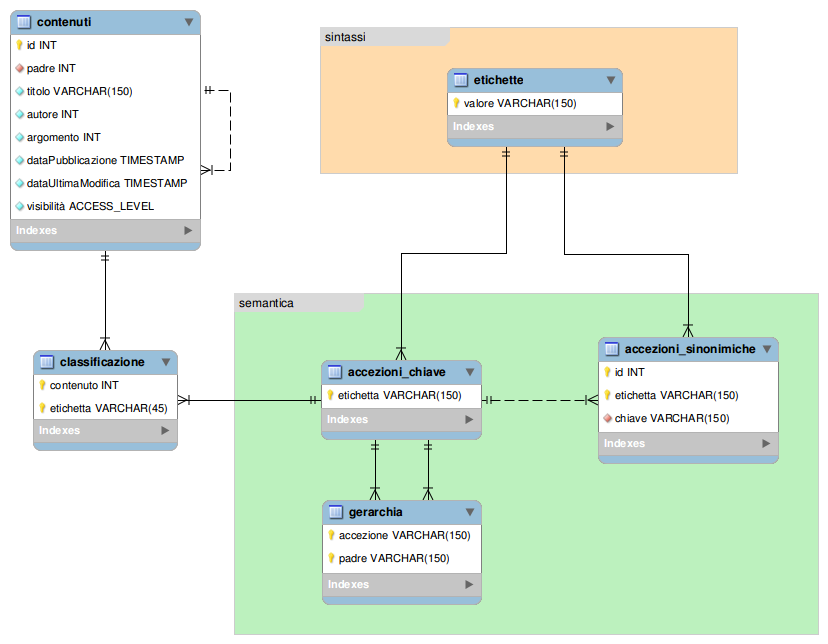
\includegraphics[width=14cm]{modello-er.png}
			\label{gfx:schema-relazionale}
			\caption{Scherma relazionale del sistema di classificazione}
		\end{center}
	\end{figure}

	\begin{itemize}
	\item separazione sintassi/semantica;
	\item evitare necessità di JOIN tra tabelle per il maggior numero possibile di operazioni.
	\end{itemize} 

	\section{Entit\`a}
	\section{Etichette}
	%Ciascuna etichetta rappresenta una parola o breve espressione in grado di identificare una o più entità del dominio. 
	\section{Accezioni}
	%Le accezioni rappresentano i possibili significati di un'etichetta, cui corrispondono altrettante entità riferibili.
	\subsection{Accezioni chiave}
	\subsection{Accezioni sinonimiche}

	%----------
	% CAPITOLO
	%----------
	\chapter{Operazioni}
	\label{ch:stage:er:operazioni}
	In questo capitolo vengono illustrate le operazioni essenziali di gestione e utilizzo del sistema di classificazione progettato ed implementato secondo le specifiche descritte nella sezione \ref{ch:stage:er:schema}.

	Per ciascuna operazione, si descrive lo scopo e si fornisce il codice \textit{SQL} con cui realizzarle, motivando ove opportuno le scelte di progettazione del database e mostrando i vantaggi ottenuti.

	Di seguito si assume che le etichette rispettino un formato standard, a garanzia dell'assenza di duplicati; le variabili nel codice SQL sono riconoscibili dal prefisso '@': si tratta in generale di informazioni note al momento dell'esecuzione dell'istruzione.

	\begin{itemize}
	\item utilizzo di etichette o trigger;
	\item principio di sostituzione;
	\item individuazione accezione chiave o sinonimica (esiste già o no l'entità nel dizionario);
	\item grafo di affinità etichette;
	\item eliminazione accezione chiave e promozione sinonimica.
	\end{itemize}
	% 

	% SECTION
	\section{Etichette}
	\label{ch:stage:er:operazioni:etichette}
	Le etichette rappresentano la componente sintattica mediante la quale gli utenti interagiscono con il sistema di classificazione, catalogando e recuperando i contenuti.

	\subsection{Ricerca di un'etichetta}
	\label{ch:stage:er:operazioni:etichette:ricerca}
	Una stringa digitata dall'utente può rappresentare il prefisso di un'etichetta o l'etichetta stessa: in entrambi i casi per cercare riscontri nel dizionario è sufficiente considerare la tabella \texttt{etichette}.

	\paragraph{Corrispondenza esatta} \hfill \\
	Restituisce - ove presente - l'etichetta corrispondente alla stringa inserita.

\begin{verbatim}
SELECT *
  FROM etichette	
 WHERE valore='@etichetta'
\end{verbatim}

	\paragraph{Corrispondenza parziale} \hfill \\
	Restituisce - ove presenti - le etichette corrispondenti alla stringa inserita o di cui quest'ultima sia prefisso.

\begin{verbatim}
SELECT *
  FROM etichette	
 WHERE valore LIKE '@etichetta%'
\end{verbatim}

	\subsection{Ricerca delle accezioni di un'etichetta}
	\label{ch:stage:er:operazioni:etichette:accezioni}
	Individuata un'etichetta, è spesso necessario recuperare le relative accezioni per identificare un'entità precisa del dominio. Tale operazione richiede di consultare separatamente le tabelle \texttt{accezioni\textunderscore chiave} e \texttt{accezioni\textunderscore sinonimiche} e di unire i risultati, eventualmente ordinandoli alfabeticamente.

\begin{verbatim}
{
  SELECT entita
    FROM accezioni_chiave	
   WHERE etichetta='@etichetta'
}
UNION
{
  SELECT entita
    FROM accezioni_sinonimiche	
   WHERE etichetta='@etichetta'
}
ORDER BY entita
\end{verbatim}

	\subsection{Ricerca dell'etichetta primaria}
	\label{ch:stage:er:operazioni:etichette:ricerca-primaria}
	Se l'etichetta inserita dall'utente risulta - rispetto ad un'accezione - secondaria, è necessario risalire alla corrispondente primaria. Ciò richiede di consultare le tabelle \texttt{accezioni\textunderscore chiave} e \texttt{accezioni\textunderscore sinonimiche}: è possibile effettuare tale operazione mediante un'unica istruzione SQL, che richiede il JOIN tra le due tabelle, o due distinte.

\paragraph{Istruzione singola}
\begin{verbatim}
SELECT c.etichetta
  FROM accezioni_chiave AS c JOIN accezioni_sinonimiche AS s
       ON (c.etichetta=s.chiave)
 WHERE s.etichetta='@etichetta' AND s.id='@id'
\end{verbatim}

\paragraph{Due istruzioni}
\begin{verbatim}
SELECT chiave
  FROM accezioni_sinonimiche	
 WHERE s.etichetta='@etichetta' AND s.id='@id'

SELECT etichetta
  FROM accezioni_chiave	
 WHERE c.etichetta='@chiave'
\end{verbatim}

	\subsection{Ricerca del numero di occorrenze di un'etichetta}
	\label{ch:stage:er:operazioni:etichette:occorrenze}
	Per determinare il numero di contenuti cui sia stata assegnata una data etichetta è sufficiente accedere alla tabella \texttt{classificazione}.

\begin{verbatim}
SELECT COUNT(*) AS num
  FROM classificazione
 WHERE etichetta='@etichetta'
\end{verbatim}

	\subsection{Inserimento di un'etichetta}
	\label{ch:stage:er:operazioni:etichette:inserimento}
	L'inserimento di una nuova etichetta si rende necessario qualora un utente cerchi di riferire un'entità con una stringa (parola o breve espressione) non presente nel dizionario (vedi sezione \ref{ch:stage:er:operazioni:etichette:ricerca-primaria}).

	A questo punto l'etichetta viene inserita nella tabella \texttt{etichette}:
\begin{verbatim}
INSERT INTO etichette
     VALUES (@stringa,current_timestamp)
\end{verbatim}

	Infine si deve associarle almeno un'accezione, che chiarisca l'entità cui si riferisce: tale operazione può essere svolta dall'utente o in maniera (semi)automatica, mediante l'assegnazione di valori predefiniti.\footnote{L'assegnazione automatica dell'accezione è possibile solo per la prima.}

	Di seguito si assume che l'utente abbia stabilito se si tratti di etichetta primaria (identifica una nuova entità) o secondaria (identificatore alternativo per un'entità definita).

	\paragraph{Accezione chiave} \hfill \\
	Se l'etichetta è primaria, si fornisce una descrizione dell'entità in questione.
\begin{verbatim}
INSERT INTO accezioni_chiave
     VALUES (@etichetta,@descrizione_entità)
\end{verbatim}

	\paragraph{Accezione sinonimica} \hfill \\
	Se l'etichetta è secondaria, è necessario indicare la corrispondente accezione chiave.
\begin{verbatim}
# i-esima eccezione sinonimica dell'etichetta @etichetta
INSERT INTO accezioni_sinonimiche
     VALUES (i,@etichetta,@accezione_chiave)
\end{verbatim}

	\subsection{Eliminazione di un'etichetta}
	Il processo di eliminazione di un'etichetta richiede di prendere in esame ciascuna accezione ed eliminarla, secondo le modalità specificate nella sezione \ref{ch:stage:er:operazioni:accezioni:eliminazione}.

	Solo una volta cancellate le relative accezioni, è possibile procedere all'eliminazione dell'etichetta dal dizionario.
\begin{verbatim}
DELETE FROM etichette
      WHERE valore=@etichetta
\end{verbatim}

	% SECTION
	\section{Accezioni}
	\label{ch:stage:er:operazioni:accezioni}
	\subsection{Aggiunta di un'accezione}
	\subsubsection{Accezione chiave}
	\subsubsection{Accezione sinonimica}
	\subsection{Eliminazione di un'accezione}
	\label{ch:stage:er:operazioni:accezioni:eliminazione}
	\subsubsection{Accezione chiave}
	Aggiornamento con etichetta sinonimica (select + update + delete)
	\subsubsection{Accezione sinonimica}

	% SECTION
	\section{Entit\`a}
	Ciascuna entità è identificata univocamente nel sistema di classificazione da un'accezione chiave e - sul piano sintattico - dalla relativa etichetta primaria. Per tale motivo la maggior parte delle operazioni coinvolge le tabelle \texttt{accezioni\textunderscore chiave} e \texttt{gerarchia}.
 
	\subsection{Ricerca dei figli}
	La ricerca dei figli di un'entità consiste banalmente nell'individuare le entità di cui essa sia il padre.
\begin{verbatim}
SELECT etichetta
  FROM gerarchia
 WHERE padre='@etichetta'
\end{verbatim}

	\subsection{Ricerca dei padri}
	La ricerca dei padri di un'entità risulta immediata e analoga alla precedente.
\begin{verbatim}
SELECT padre
  FROM gerarchia
 WHERE etichetta='@etichetta'
\end{verbatim}

	\subsection{Ricerca delle etichette}
	Per ottenere la lista completa delle etichette con cui è riferibile una determinata entità del dominio, è sufficiente recuperare l'etichetta primaria e - a partire da questa - le etichette sinonimiche.

	\paragraph{Etichetta primaria}
\begin{verbatim}
SELECT etichetta
  FROM accezioni_chiave
 WHERE entita='@entita'
\end{verbatim}

	\paragraph{Etichette sinonimiche}
\begin{verbatim}
SELECT etichetta
  FROM accezioni_sinonimiche
 WHERE padre='@etichetta'
\end{verbatim}

	\subsection{Aggiungere una relazione padre-figlio}
	L'aggiunta di un una relazione padre-figlio tra entità esistenti richiede di specificare padre e figlio nella tabella \texttt{gerarchia}.
\begin{verbatim}
INSERT INTO gerarchia(etichetta,padre)
     VALUES (@figlio,@padre)
\end{verbatim}
	
	%\subsection{Controllo di assenza cicli}

	% SECTION	
	\section{Contenuti}
	\subsection{Assegnazione di un'etichetta}
	L'assegnazione di un'etichetta (più precisamente un'accezione chiave) ad un contenuto assume che sia stata individuata l'etichetta primaria per l'entità in questione (v. sezioni \ref{ch:stage:er:operazioni:etichette:ricerca} e \ref{ch:stage:er:operazioni:etichette:accezioni}). A questo punto si procede inserendo una nuova riga nella tabella \texttt{classificazione}.
\begin{verbatim}
INSERT INTO classificazione(contenuto,etichetta)
     VALUES (@contenuto,@etichetta)
\end{verbatim}

	\subsection{Ricerca delle etichette assegnate}
	Il reperimento della lista delle etichette primarie	assegnate ad un contenuto richiede di consultare la tabella \texttt{classificazione}.
\begin{verbatim}
SELECT etichetta
  FROM classificazione
 WHERE contenuto='@contenuto'
\end{verbatim}

	%Il numero di contenuti trovati esprime l'attinenza delle etichette, ossia quanto vengano usate insieme 
	\subsection{Ricerca di contenuti generici}
	La ricerca dei contenuti cui sia stata assegnata una certa etichetta richiede di consultare la tabella \texttt{classificazione}.
\begin{verbatim}
SELECT contenuti
  FROM classificazione
 WHERE etichetta='@etichetta'
\end{verbatim}

	\subsection{Ricerca di contenuti specifici}
	La ricerca di contenuti specifici consiste nell'individuare i contenuti cui siano state assegnate - tra le altre - determinate etichette (due o più) specificate dall'utente. 
\begin{verbatim}
  SELECT contenuto, COUNT(etichetta)
    FROM classificazione
   WHERE etichetta='@etichetta1' [OR etichetta='@etichetta2' ...]
GROUP BY contenuto
  HAVING COUNT(*)>=@num_etichette
\end{verbatim}

	%\subsection{Principio di sostituzione}

\end{document}
